\documentclass{beamer}

\usepackage{default}

\usetheme{Rochester}
\usecolortheme{beaver}

\title{Extensions on Contract Net Protocol for AGVs}
\subtitle{Multi-Agent Systems}

\author{Jens Claes \and Victor Le Pochat}
\date{June 6, 2016}

\begin{document}
	\frame{\titlepage}

	\begin{frame}{Objectives \& Hypotheses}
		\begin{itemize}
		\item Investigate two extensions on CNET: CNCP and DynCNET
		\item Setting: PDP with drones
		\item Hypotheses:
			\begin{itemize}
			\item Profit comparison
			\item Influence of drones/clients/warehouses on profit
			\item Delivery time comparison
			\item \# clients undelivered
			\item Message count comparison
			\end{itemize}
		\end{itemize}
	\end{frame}
	\note{Hypotheses zelf gewoon zeggen}

	\section{Theory}
	
	\begin{frame}{Contract Net Protocol (CNET)}
		\begin{itemize}
			\item Assigning tasks to (idle) agents
			\item Distributed manner
			\item Contract negotiation between manager and contractor
			\begin{itemize}
				\item M: Task announcement
				\item C: Bid
				\item M: Awarding
				\item C: Execution
			\end{itemize}
		\end{itemize}
	\end{frame}
	
	\begin{frame}{Contract Net Protocol (CNET)}
	  \begin{columns}[T] % the "c" option specifies center vertical alignment
	  \column{.5\textwidth} % column designated by a command
	   Negotiation protocol
	  \column{.5\textwidth}
	   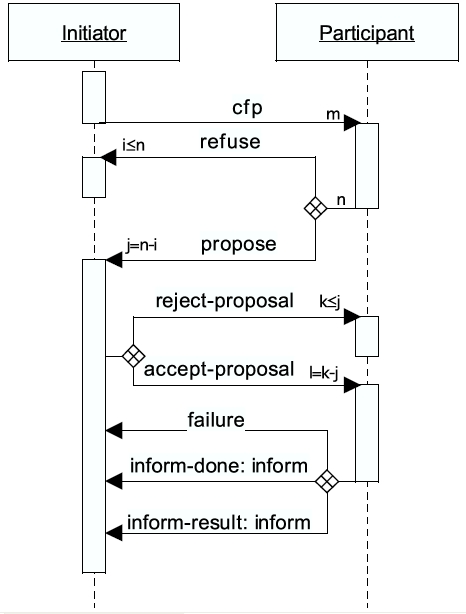
\includegraphics[width=\columnwidth]{FIPA-CNET}
	  \end{columns}
	\end{frame}

	\begin{frame}{Contract Net with Confirmation (CNCP)}
		\begin{itemize}
			\item CNET problem: early commitment
			\item CNCP solution: full commitment when awarded
			\item Contractor submits bid but continues bidding
			\item When awarded, first check if contractor accepts
			\begin{itemize}
				\item if yes: award \& execute task
				\item if no: try next best contractor
			\end{itemize}
		\end{itemize}
	\end{frame}

	\begin{frame}{Dynamic Contract Net (DynCNET)}
		\begin{itemize}
			\item CNET problem: no dynamism
			\item DynCNET solution: allow contract switching
			\item When awarded but still in preparation
			\item Contract final when preparation is finished
		\end{itemize}
	\end{frame}
	
	\begin{frame}{MAS design}
		\begin{itemize}
			\item
		\end{itemize}
	\end{frame}
	
	\begin{frame}{MAS design comparison}
		\begin{itemize}
			\item
		\end{itemize}
	\end{frame}
	
	\begin{frame}{Experiments}
		\begin{itemize}
			\item
		\end{itemize}
	\end{frame}
	
	\begin{frame}{Conclusion}
		\begin{itemize}
			\item
		\end{itemize}
	\end{frame}
	
\end{document}
